\documentclass[english]{article}

%I think these are useful for pdftex compatibility. I bastardised an old latex report.
\usepackage[T1]{fontenc}
\usepackage[utf8]{inputenc}

\usepackage[a4paper]{geometry}

%for manual adjustment of borders if necessary
\usepackage{verbatim}
\usepackage{algorithm,algorithmic}
\usepackage{amsthm}
\usepackage{amsmath}
\usepackage{amsfonts}
\usepackage{graphicx}
\usepackage{fixltx2e}
\usepackage{stfloats}
\usepackage{subfig}
\usepackage{babel}
\usepackage{float}

\begin{document}

\title{Statistical methods in perception and their application to the SLAM problem}

\author{Duncan Burke and Sebastian Pauka}
\maketitle

\begin{abstract}
Given the inherent uncertainty of any sensor, filtering is a central issue in the problem of reliable robot perception. Statistical methods have become central to any perception problem. The following report evaluates two common classes of filter, the Kalman Filter and the Particle Filter, in a variety of situations, and uses insights gained to implement the FastSLAM algorithm for mapping.
\end{abstract}

\section{Introduction}
A fundamental requirement for any robotics system is the ability to perceive and interact with its physical environment. Any reasonable interaction of a robot with its environment requires an internal model of its surroundings for purposes such as robot localisation, map generation, planning and to enable any other sensor processing to be placed in its spatial context. The creation of this model requires \emph{data fusion} - some algorithm  enabling a multitude of data sources and measurements to produce a unified estimate. It must also be considered that the data incorporated into such a model is inherently noisy and may further suffer from systematic error, and that in realistic applications algorithmic approximations are commonly necessary for computational tractability \cite{probrob}.

This data fusion is accomplished through the use of filters. At their core, filters combine observable processes such as sensor data and knowledge about what the robot is doing into a model of its surroundings, representing the \emph{state} of the robot. Two common filters are addressed in this report: the Kalman Filter and the Particle filter.

The use of statistical filters has been particularly successful in attempting to solve two of the largest problems in robotics, localization and mapping. The term localization encompasses a number of problems. In order of increasing difficulty, a full treatment of localization implies solutions to the problems of:
\begin{enumerate}
 \item \emph{Position Tracking} - in which the initial position of the robot is known, and hence only keeping track of the motion is required.
 \item \emph{Global Localization} - in which the initial position is not known and must be determined from sensor inputs.
 \item \emph{Kidnapped Robot Problem} - in which a robot's position may be changed without its knowledge, hence the change must be detected and position must be recalculated. This problem is different to the Global Localization problem in that the robot does not know that it's position is indeterminate. With the knowledge that localization could fail (leading to an erroneous position determination), a full treatment of the localization problem should be able to solve the Kidnapped Robot Problem and hence recover from global localization failures \cite[pp 193-196]{probrob}.
\end{enumerate}

Note that the treatment of the localization problems in this report assumes that a passive approach with a single robot.

With reference to the algorithms that have been studied previously, there are several algorithms which solve the Kidnapped Robot Problem, including Multi Hypothesis Tracking (MHT), which utilises an Unscented Kalman Filter to represent a number of possible positions, and Monte Carlo Localization (MCL) which utilises Particle Filters to perform localization \cite[pp 274]{probrob}. The report gives a rigorous treatment of MCL to the kidnapped robot problem.

Considering now the mapping problem, there are again a number of problems which must be solved to perform mapping. In particular, in this report, we consider the Simultaneous Localization and Mapping (SLAM) problem, which assumes uncertainty in both the location and the sensor measurements in constructing a map. In order for a full solution to this problem, it must simultaneously handle localization errors by correcting position estimates with the map, while constructing the map using position estimates. The circular nature of the problem makes it one of the most difficult in the field of robotics.

One of the most popular algorithms for solving the SLAM problem is the FastSLAM algorithm, which at a high level, utilizes particle filters to represent a number of candidate maps constructed off uncertain position estimates and selects those maps which best fits observations. In this report, an algorithm for performing FastSLAM is described and evaluated.

\section{Background}

\subsection{Filtering Algorithms}
\label{sec:filtering}
There has been a lot of effort placed into developing statistical methods for filtering information. Recent developments in robotics have focused on exploiting the statistical nature of the uncertainty of measurement to derive some internal state from a variety of sensory and command inputs.

The internal state is given in discrete steps by the variable $x_t$, indexed by time $t$. In addition, at time $t$, control data $u_t$ and measurements $z_t$ are received. It is assumed that commands and measurements occur in discrete steps with the measurement $z_t$ taken after the preceding control command given by $u_t$ has been completed. The state $x_t$ is not directly observable and must be generated stochastically from the previous states $x_{0:t-1}$, movement commands $u_{1:t-1}$ and sensor inputs $z_{0:t}$ \cite{Thrun02d}. If $x_t$ is conditionally independent of $x_{0:t-2}$ and $u_{1:t-2}$ given $x_{t-1}$, x is said to be \emph{complete} and satisfies the \emph{Markov Condition}\cite{probrob}. Although $x_t$ is hidden, the measurement $z_t$ is generated stochastically from $x_t$ allowing for indirect observation\cite{Thrun02d}.

The belief distribution $bel(x_t)$ of the state $x_t$ assigns a probability to every possible state that it is the actual hidden state. The belief is defined conditionally on all past movement commands and sensor measurements (Equation \ref{eq:bel}) \cite{probrob}. It is also convenient to define the belief in $x_t$ prior to incorporating the measurement $z_t$ generated from $x_t$ (Equation \ref{eq:prediction}); this is referred to as the \emph{prediction} and is used to generate $bel(x_t)$ by incorporating $z_t$ in a \emph{measurement update}.
\begin {align}
  bel(x_t) & = p(x_t \mid z_{1:t},u_{1:t}) \label{eq:bel} \\   
  \overline{bel}(x_t) & = p(x_t \mid z_{1:t-1}, u_{1:t}) \label{eq:prediction}
\end {align}

The following methods generally assume the Markov Condition, namely the assumption that past and future states are independent if the current state is known. In other words, all future states should be able to be extrapolated from complete knowledge of the present state. This represents a very strict precondition, and in practice, due to a number of factors such as unmodeled dynamics (factors of the environment not taken into account), inaccuracy of the models etc. it is impossible to completely satisfy this condition. Therefore any method that assumes the Markov condition must also be relatively robust against violations of the condition since it is impossible for the Markov condition to be completely satisfied in practice \cite[pp 33]{probrob}.

\subsubsection{Bayes Filter}

% Define complete here...

The Bayes Filter is an algorithm used to calculate the belief $bel(x_t)$. It is assumed that the state is complete, and therefore satisfies the Markov condition. Therefore, the algorithm can be framed recursively as an \emph{update rule} calculating the new belief $bel({x_t})$ given the previous belief $bel(x_{t-1})$ and new inputs $u_t$ and $z_t$. The algorithm consists of two core steps: the \emph{control update} and the \emph{measurement update}. Firstly, for every state $x_t$ in the state space, an updated prediction $\overline{bel}(x_t)$ is given by the integral of the conditional probability of $x_t$ given $bel(x_{t-1})$ and $u_t$\cite{probrob}. This requires the \emph{movement model} $p(x_t \mid u_t,x_{t-1})$ and may be given by a direct summation in the case of a discrete state space. $bel(x_t)$ can be calculated from the \emph{measurement model} $p(z_t \mid x_t)$ and $\overline{bel}(x_t)$ through a single application of Bayes' Theorem.

\begin{algorithm}[H]
\caption{Bayes Filter}
\label{alg:bayes}
\begin{algorithmic}
	\REQUIRE $bel(x_{t-1}), u_t, z_t$
        \FOR {all $x_t$}
        \STATE $\overline{bel}(x_t) \leftarrow \int p(x_t \mid u_t, x_{t-1})bel(x_{t-1}) dx_{t-1}$
        \STATE $bel(x_t) \leftarrow \eta p(z_t \mid x_t) \overline{bel}(x_t)$
        \ENDFOR
        \RETURN $bel(x_t)$
\end{algorithmic}
\end{algorithm}

However, this algorithm is intractable in all but the simplest of scenarios, requiring a sum over the entire state space for all $x_t$. For continuous random variables, this is accomplished via an integral which in general, does not necessarily have an analytic solution. For finite state spaces, this is accomplished via a summation over the state space, which may, too be impractically computationally expensive. On the other hand, the normalisation of the measurement update $\eta$ is easily calculated as a summation over the unnormalised posterior, as the posterior is calculated for all $x_t$.

It is, however, possible to simplify or approximate the algorithm given certain restrictions on the input. Both the Kalman and Particle Filters provide practical implementations of the Bayes Filter by making suitable assumptions or approximations.

\subsubsection{Kalman Filter}
\label{sec:kalfilter}
One of the most common implementations of the Bayes filter is the Kalman Filter. It is structurally very similar to Hidden Markov Model, however with the nodes being real valued vectors and the probability model being Gaussian \cite{kalfilter}. It is one of the most studied filtering techniques for a number of reasons, including its simplicity and efficiency.

The filter relies on a number of assumptions about the inputs, above those made by the Bayes' Filter, namely:
\begin{enumerate}
	\item The state transition probability $P(x_{t} \mid u_t,x_t)$ is a linear function with added Gaussian noise. A linear Gaussian is expressed as:
		\begin{equation}
			x_{t} = A_{t} x_{t-1} + B_{t} u_{t} + \epsilon _{t}
		\end{equation}
		Since $A_{t}$ and $B_{t}$ are constant, the state transition function is linear in its arguments. The noise is a multivariate Gaussian with mean zero and covariance $R_t$.
	\item The measurement probability must also be linear in its arguments, again with added Gaussian nose. It is expressed as:
		\begin{equation}
			z_{t} = C_{t} x_{t} + \delta _{t}
		\end{equation}
		The value $\delta_t$ gives measurement noise (i.e. an estimate of the uncertainty of the sensors), and is a multivariate Gaussian with a mean of zero and covariance $Q_t$.
	\item The initial belief $bel(x_0)$ must be normally distributed. This is denoted:
		\begin{equation}
			bel(x_0) = P(x_0) \sim \mathcal{N}(\mu_0, \Sigma_0)
		\end{equation}
		such that the initial belief is $bel(x_0)=\mu_0$.
\end{enumerate}
Under these assumptions, we can show that for any $t$, the posterior $bel(x_{t})$ is always Gaussian \cite{kalmanderiv}.

In the following discussion, the terms $bel(x_t)$ and $\mu_t$ will be used interchangeably to indicate the current state of the belief.

The constant terms of the state transition probability, $A_{t}$ and $B_{t}$ are matrices which represent some physical relationship between the terms of the state vector ($x_{t-1}$) and the control vector ($u_{t}$). As such, if the dimension of the state vector is $n$ and the dimension of the control vector is $m$ then the matrix $A_{t}$ is a $n \times n$ matrix, and the matrix $B_{t}$ is a $n \times m$ matrix, such that the posterior state vector is also a vector of dimension $n$. 

The random variable $\epsilon _{t}$ is a Gaussian random vector of dimension $n$ that represents the uncertainty introduced by the state transition. It has a mean of zero, and covariance $R_{t}$.

The filter runs in two stages, the time update and the measurement update. In the time update stage, with the knowledge that the mean represents the most likely state, and the covariance the uncertainty in the state, we want to calculate a new distribution conditioned on the measurement vectors $(z_0, z_1, ..., z_{t-1})$, in other words, not utilizing the new measurement vector. We can express this as the following, where $\overline{\mu}_{t}$ represents the mean and $\overline{\Sigma}_{t}$ represents the covariance. To summarize, by definition \cite{kalfilter}:
\begin{eqnarray}
\label{eq:postmean}
\overline{\mu}_{t} &\equiv& E\left[x_{t} \mid z_0,...,z_{t-1}\right] \\
\label{eq:postvar}
\overline{\Sigma}_{t} &\equiv& E\left[(x_{t} - \overline{\mu}_{t})(x_{t} - \overline{\mu}_{t})^T \mid z_0,...,z_{t-1}\right]
\end{eqnarray}

Considering first the time update, we simply propagate the distribution forward one step in time, calculating a new mean and covariance based on the old mean and covariance, without considering measurements. The mean is simply found by calculating the linear expression for the state transition probability ($A_{t} x_{t-1} + B_{t} u_{t} + \epsilon_{t}t$). We can find that the covariance is given by definition (eq. ~\ref{eq:postvar}) to be:
\begin{equation}
\overline{\Sigma}_{t} = A_{t} \Sigma_{t-1} A_{t}^T + R_{t}
\end{equation}

In the measurement update step, we need to calculate the conditional mean and covariance of $y_{t+1}$, and the conditional covariance of $x_{t+1}$ and $y_{t+1}$. Knowing this we can write the joint conditional distribution of $x_{t+1}$ and $y_{t+1}$. We can then just reverse the process using the definitions of the Bayes distribution. We find then that the end result is:
\begin{eqnarray}
\mu_{t} &=& \overline{\mu}_{t} + \overline{\Sigma}_{t} C_{t}^T (C_{t} \overline{\Sigma}_{t} C_{t}^T + Q_t)^{-1}C_t (z_{t} - C_{t} \overline{\mu}_{t}) \\
\Sigma_{t} &=& \overline{\Sigma}_{t} - \overline{\Sigma}_{t} C_{t}^T (C_{t} \overline{\Sigma}_{t} C_{t}^T + R_{t})^{-1}C_{t} \overline{\Sigma}_{t}
\end{eqnarray}

We define the term in $\mu_{t+1}$ to be the Kalman Gain, or the amount that the measurement is integrated into the new belief, such that \cite{probrob}:
\begin{equation}
K_{t} = \overline{\Sigma}_{t} C_{t}^T (C_{t} \overline{\Sigma}_{t} C_{t}^T + Q_t)^{-1}C_{t}
\end{equation}

The algorithm for the Kalman filter is thus: \cite{probrob}

\begin{algorithm}[H]
\caption{Kalman Filter}
\label{alg:kalman}
\begin{algorithmic}[1]
	\REQUIRE $\mu_{t-1}, \Sigma_{t-1}, u_t, z_t$
	\STATE $\overline{\mu}_t \leftarrow A_t\mu_{t-1} + B_t \mu_t$
	\STATE $\overline{\Sigma}_t \leftarrow A_t \Sigma_{t-1}A_t^T + R_t$
	\STATE
	\STATE $K_t \leftarrow \overline{\Sigma}_t C_t^T\left(C_t \overline{\Sigma}_t C_t^T + Q_t\right)^{-1}$
	\STATE $\mu_t \leftarrow \overline{\mu}_t + K_t\left(z_t - C_t \overline{\mu}_t\right)$
	\STATE $\Sigma_t \leftarrow (I-K_t C_t)\overline{\Sigma}_t$
	\RETURN $\mu_t, \Sigma_t$
\end{algorithmic}
\end{algorithm}

The new belief is thus represented by $bel(t) = \mu_t$ with covariance $\Sigma_t$. We notice that in using the previous belief $bel(t-1)$ in place of the hidden state, we need only to consider the measurement variable of the new state, without considering previous measurements.

By substitution of $\mu_t$ and $\Sigma_t$ into the definition of the multivariate Gaussian distribution, we can find the probability distribution of the state space.

It is interesting to note that the Kalman filter can be interpreted as a LMS error correcting algorithm. We can through simplification of the Kalman filter find that it is functionally equivalent to the LMS algorithm.

\subsubsection{Particle Filter}

%Overview of a particle filter - state represented as a sampling of possible states
Whereas the Kalman Filter represents the belief as a parameterised Gaussian distribution, the Particle Filter is non-parameterised, representing the belief at time $t$ as a finite set $\chi_t$ of $M$ states $\{x^{[1]}_t, x^{[2]}_t, \cdots , x^{[M]}_t\}$ drawn from the state space according to the distribution of the posterior. By increasing the number of particles, $\chi$ can be made to asymptotically approximate any distribution without any regards to constraints such as uni-modality\cite{Thrun02d}.

At the start of the algorithm, the set of particles $\chi_0$ are drawn according to the distribution of the start state $p(x_0)$ (Equation \ref{eq:particle_initial}). At time $t$, a single new hypothetical state $x^{[m]}_t$ is generated from each particle $x^{[m]}_{t-}$ for $m \in [1,M]$ by sampling a state from the distribution of the state transition probability (Equation \ref{eq:particle_prediction}). These new states belong to $\bar{\chi}_t$ which is distributed according to the predicted belief $p(x_t \mid u_t,x^{[m]}_{t-1})$.

From the Bayes Filter (Algorithm \ref{alg:bayes}), $bel(x_t) = \eta p(z_t \mid x_t) \overline{bel}(x_t)$. To produce the desired target distribution from $\bar{\chi}_t$ according to this relationship, $\bar{\chi}_t$ must be resampled with each particle weighted by the measurement model $p(z_t \mid x_t)$. For each $x^{[m]}_{t}$, a weight $w^{[m]}_t$ is calculated (Equation \ref{eq:particle_weight}). Next, a re-sampling step randomly selects with replacement $M$ particles from $\bar{\chi}_t$ into $\chi_t$ with each particle $x^{[m]}_{t}$ weighted by $w^{[m]}_t$ given by the measurement model\cite{probrob}.

\begin {align}
  x^{[m]}_0 \sim  p(x_0) \label{eq:particle_initial}\\
  x^{[m]}_t \sim p(x_t \mid u_t,x^{[m]}_{t-1}) \label{eq:particle_prediction} \\
  w^{[m]}_t = \eta p(z_t \mid x^{[m]}_t) \label{eq:particle_weight}
\end {align}

Hence, the complete algorithm is:
\begin{algorithm}
\caption{Particle Filter}
\label{alg:particle}
\begin{algorithmic}
	\REQUIRE $\chi_{t-1}, u_t, z_t$
        \STATE $\bar{\chi}_t = \chi_t = \emptyset$
        \FOR {$m \leftarrow 1$ to $M$}
        \STATE sample $x^{[m]}_t \sim p(x_t \mid u_t,x^{[m]}_{t-1})$
        \STATE $w^{[m]}_t \leftarrow p(z_t \mid x^{[m]}_t)$
        \STATE Add $\left\langle x^{[m]}_t, w^{[m]}_t \right\rangle$ to $\bar{\chi}_t$
        \ENDFOR

        \FOR {$m = 1$ to $M$}
        \STATE Select an index $i \in [1,m]$ with probability $\propto w^{[i]}_t$
        \STATE Add $\left\langle x^{[i]}_t \right\rangle$ to $\chi_t$
        \ENDFOR

\end{algorithmic}
\end{algorithm}

It can be shown through induction on Bayes' Rule that $bel(x_{0:t})$ can be given by Equation \ref{eq:particle_equation}.
\begin{align}
  bel(x_{0:t}) & = \eta w^{[m]}_tp(x_t \mid x_{t-1}, u_t)p(x_{0:t-1} \mid z_{0:t-1},u_{0:t-1}) \label{eq:particle_equation}
\end{align}
Following this algorithm, asymptotically $\underset{M \to \infty}{\lim} x^{[i]}_t \sim p(x_t \mid z_{1:t}, u_{1:t})$.

Generally speaking, while the particle set itself represents the posterior $p(x_t \mid z_{1:t}, u_{1:t})$, for many purposes such as planning, it is desirable to produce a state estimation in a more useful form. The simplest such method builds a discrete histogram over the state space, with the occupancy of each bin approximating the posterior density at its position. Alternatively, a Gaussian approximation could provide an effective maximum likelihood representation if the posterior is unimodal. In the case of multimodal posteriors, k-means clustering may be used to provide a multimodal approximation as a mixture of multiple Gaussians\cite{probrob}.
\subsection{Localization}
We will now leverage the kalman and particle filters to solve the localization problem. The first assumption in this problem is that a map or set of known features is available. This map could be created through other means, such as survey equipment, aerial photos, or another robot having mapped the environment through SLAM. Secondly, models must be available to produce the functions specified in algorithms \ref{alg:particle} and \ref{alg:kalman}. Which models are required and the form of the models is dependent on the problem; for example, the EKF requires that the Jacobian of the functions be readily available.

In most localization problems, two distinct types of models are required: a model representing the kinematics of the robot and models representing the various sensor measurements. 

For simplicity, only the kinematic problem of a robot in the plane was examined. In this case, the pose of the robot is represented by the vector $x_t = (x,y,\theta)^T$. There are two distinct motion models that can now be used, the velocity and odometry models.
The velocity model assumes that a control instruction $u_t = (v_t, \omega_t)^T$ consists of a forward velocity $v_t$ and a rotational velocity $\omega_t$. The path of the robot within a single timestep can then be described by an arc of a circle with uncertainty in the  velocity, angular veloctity and final orientation \cite{probrob}. Note that the function $\textrm{sample}(\sigma)$ samples from a zero---centered distribution with standard deviation $\sigma$. Also, this model has coefficients $\alpha_{1\rightarrow 6}$ relating the uncertainty to both the angular and forwards velocity; in practice, turning can be a significant source of noise due to effects such as slipping of the wheels.

\begin{algorithm}
\caption{Velocity Motion Model}
\label{alg:velocity_model}
\begin{algorithmic}
	\REQUIRE $u_t = (v, \omega)^T, x_{t-1} = (x, y, \theta)^T $
        \STATE $\hat{v} = v + \textrm{sample}(\alpha_1|v| + \alpha_2|\omega|)$
        \STATE $\hat{v} = v + \textrm{sample}(\alpha_3|v| + \alpha_4|\omega|)$
        \STATE $\hat{\gamma} = \textrm{sample}(\alpha_5|v| + \alpha_6|\omega|)$
        \STATE $x' = x - \frac{\hat{v}}{\hat{\omega}}\sin{\theta} + \frac{\hat{v}}{\hat{\omega}}\sin{(\theta + \hat{\omega} \Delta t)}$
        \STATE $y' = y + \frac{\hat{v}}{\hat{\omega}}\cos{\theta} - \frac{\hat{v}}{\hat{\omega}}\cos{(\theta + \hat{\omega} \Delta t)}$
        \STATE $\theta' = \theta + \hat{\omega}\Delta t + \hat{\gamma}\Delta t$
        \RETURN $x_t = (x', y', \theta')^T$
\end{algorithmic}
\end{algorithm}


When a control command is sent, the motors and actuators attempt to carry it out, producing some change in the robot's pose which is then approximated by the odometry. The velocity motion model probabilistically relates the control to the change in pose, the odometry model estimates the pose from the odometry data. In practice, odometry has the significant advantage of measuring a robot's change in pose after the fact; for example, if a robot collided with an obstacle, the velocity model may optimistically assume the robot travelled through, whereas the odometry may show the robot being halted.

\begin{algorithm}
\caption{Odometry Motion Model}
\label{alg:odometry_model}
\begin{algorithmic}
	\REQUIRE $u_t = (\bar{x}_{t-1},\bar{x}_t)^T, x_{t-1} = (x, y, \theta)^T$
        \STATE $\delta_{\mathrm{rot1}} = \mathrm{atan2}(\bar{y}' - \bar{y}, \bar{x}' - \bar{x}) - \bar{\theta}$
        \STATE $\delta_{\mathrm{trans}} = \sqrt{(\bar{y}' - \bar{y})^2 + (\bar{x}' - \bar{x})^2}$
        \STATE $\delta_{\mathrm{rot2}} = \bar{\theta}' - \bar{\theta} - \delta_{\mathrm{rot1}}$
        \STATE $\hat{\delta}_{\mathrm{rot1}} = \delta_{\mathrm{rot1}} - \textrm{sample}(\alpha_1|\delta_{\mathrm{rot1}}| + \alpha_2\delta_{\mathrm{trans}})$
        \STATE $\hat{\delta}_{\mathrm{trans}} = \delta_{\mathrm{trans}} - \textrm{sample}(\alpha_4(|\delta_{\mathrm{rot1}}| + |\delta_{\mathrm{rot2}}|)+ \alpha_3\delta_{\mathrm{trans}})$
        \STATE $\hat{\delta}_{\mathrm{rot2}} = \delta_{\mathrm{rot2}} - \textrm{sample}(\alpha_1|\delta_{\mathrm{rot2}}| + \alpha_2\delta_{\mathrm{trans}})$
        \STATE $x' = x + \hat{\delta}_{\mathrm{trans}}\cos{(\theta + \hat{\delta}_{\mathrm{rot1}})} $
        \STATE $y' = y + \hat{\delta}_{\mathrm{trans}}\sin{(\theta + \hat{\delta}_{\mathrm{rot1}})} $
        \STATE $\theta' = \theta + \hat{\delta}_{\mathrm{rot1}} + \hat{\delta}_{\mathrm{rot2}}$
        \RETURN $x_t = (x', y', \theta')^T$
\end{algorithmic}
\end{algorithm}

The primary form of measurement examined was a laser rangefinder. While lasers have a high degree of accuracy, there is nonetheless noise, both from the sensor itself and from spurious measurements. Furthermore, laser rangefinders have a maximum range, though in some cases this may safely be ignored. 

\subsection{The SLAM Problem}
Having defined a number of algorithms for performing filtering and localization, we would now like to combine all the previous information into a statistical method for constructing a map. Given that we know that both position information and scan information is uncertain, we would like to some how construct a map which combines the uncertainties of all control and sensor measurements to create a statistically most likely map.

Construction of a map represents one of the most difficult problems in the field of robotics as there is a circular dependency which occurs in this process. Namely, construction of the map depends on a certain position, however the position depends on the correlation of observations with the map. With this in mind, it is possible to define two classes of the SLAM problem:
\begin{enumerate}
 \item \emph{Online SLAM Problem} - Wherein the posterior and the map is estimated over the momentary pose. In other words, only the current pose $x_t$ is used to calculate the map $m$ and correspondence variables $c_t$:
	\begin{equation}
	 p\left(x_t, m, c_t | z_{1:t}, u_{1:t}\right)
	\end{equation}
	Often the previous measurement and control are forgotten after the measurement is incorporated, potentially making the online SLAM problem more efficient than the Full SLAM Problem. In addition, the result of the online SLAM problem is the result of integrating all past posses one at a time, leading to interesting dependencies between measurements which may lead to an error which must be accounted for. However, this does have the advantage of building a map as the robot navigates, of which control decisions can be made. Any autonomous mapping algorithm would be expected to solve the full SLAM problem.
 \item \emph{Full SLAM Problem} - Wherein the posterior and map is estimated over the entire path $x_{1:t}$ along with the map:
  \begin{equation}
   p\left(x_{1:t}, m, c_{1:t} | z_{1:t}, u_{1:t}\right)
  \end{equation}
  While a solution Full SLAM Problem may lead to more accurate results in some circumstances, due to its ability to propagate pose uncertainties back through the full construction as new data is incorporated, measurements must be completed before a map can be constructed making it unsuitable for the construction of maps on the fly, and decision making processes on incomplete maps.
\end{enumerate}

Therefore, there are two separate issues which must be addressed to solve the SLAM problem. The first is the representation of the map, the second, how to simultaneously represent the uncertainty in the posterior and the measurement while making usable approximations out of both of these values. 

Here, we deal exclusively with the occupancy grid representation of a map as opposed to a feature based representation, which represents map positions in a grid, labelled either occupied or unoccupied (with corresponding uncertainties). 

\subsubsection{Occupancy Grids}
The ocuupancy grid representation of a map generally encodes a 2 dimensional slice of observations, using a fine grained grid to represent occupancy. Due to this fact, the dimensionality of the map increases with the size of the map squared (i.e. area), and thus the dimensionality of a map is generally very high, meaning it is infeasible to calculate the probability of each individual map out of the set of all possible maps. For example, given a side length of 100 cells, the total number of cells is $100^2$ and the total number of possible maps is $2^{100^2}$. However, we can calculate the probability of a map as the probability over each of its cells, each of which encode a binary state:
\begin{equation}
p\left(m | z_{1:t}, x_{1:t}\right) = \prod_i p\left(\textbf{m}_i | z_{1:t}, x_{1:t}\right)
\end{equation}

Note that we assume that the pose $x_{1:t}$ is assumed to be certain. 

By this representation, the probability is given as a binary estimation problem with static state. We note also that that the probability of cells being occupied or otherwise is often close to zero, Because of this it may be more approriate to use the log odds representation for the probability of occupancy:
\begin{equation}
l_{t,i} = \log{\frac{p(\textbf{m}_i | z_{1:t}, x_{1:t})}{1-p(\textbf{m}_i | z_{1:t}, x_{1:t})}}
\end{equation}

The final observation we make is that the probability of occupancy is only likely to change if a measurement is made in the field of observation for the robot in its current state. This significantly decreases the number of cells which must be updated.

The full algorithm for creating an occupancy grid is thus given by algorithm ~\ref{alg:occgrid}.

\begin{algorithm}
\caption{Occupancy Grid Mapping}
\label{alg:occgrid}
\begin{algorithmic}
	\REQUIRE $m_{t-1}, x_t, z_t$
	\FOR {all $\textbf{m}_{t-1,i}$ in $m_{t-1}$}
	\IF {$\textbf{m}_{t-1,i}$ in perceptual field of $z_t$}
	\STATE {$\textbf{m}_{t, i} \leftarrow \textbf{m}_{t-1,i} + \textbf{inverse\_sensor\_model}\left(m_{t-1,i}, x_t, z_t\right) - l_0$}
	\ELSE
	\STATE $\textbf{m}_{t, i} \leftarrow \textbf{m}_{t-1, i}$
	\ENDIF
	\ENDFOR
	\RETURN $m_t$
\end{algorithmic}
\end{algorithm}

The function \textbf{inverse\_sensor\_model} is dependant on the sensor data and thus cannot be defined in general.

\subsubsection{FastSLAM}
The FastSLAM algorithm, and its later deriviatives such as DP-SLAM and DP-SLAM 2.0, are amongst the most successful algorithms in solving the SLAM problem, both in terms of accuracy and speed. The key feature of the SLAM problem that allows the use of particle filters, which scale exponentially with dimension, making their use unsuitable for highly dimensional data such as occupancy grids, is that there is conditional independance of between features on a map given the robot pose. In other words, if we know the exact position of the robot, then each of the scanned beams, in the case of a laser range finder, are independant of each other, as we would intuitively expect.

As such, we can factor the map as for each of the particles, due to the fact that the individual map errors are conditionally independant of each other. This property means that we can overcome the problem of the high dimensionality of the representation therefore making the particle filter efficient enough for use in mapping.

The form of particle filters we apply to the problem are known as Rao-Blackwellized particle filters, based on the work of Rao(1945) and Blackwell(1947) in computing distributions over sets of variables by combining parametric density functions.

The algorithm as described can be used in both feature based and occupancy grid based mapping algorithms. The following discussion focuses exclusively on the occupancy grid mapping approach.

The core idea of the particle filter algorithm is that each particle describes a robot pose, and in the construction of the map, it is assumed that the robot pose is described by each particle with complete accuracy. This approach solves the earlier problem of the position depending on the map, and the map depending on the position as uncertainty in the position is represented by a diversity of particles, and hence is not factored into the generation of the map. Particles are then selected by the process of importance resampling as defined in the algorithm ~\ref{alg:particle}.

The strength of the FastSLAM algorithm comes from the fact that data associations are stored per particle, and as such the algorithm stores a map per possible path making it much more robust to data association problems. This is in contrast to other common algorithms used for mapping, such as SLAM with EKF's, GraphSLAM or SEIF, where a map is only stored for the most likely track. In addition, since the particle filter does not rely on a linear motion and measurement model (or even a linearisable model), complicated non-linear models can bbe used with particle filters to build a map.

It is interesting to note that the FastSLAM algorithm solves both the Online SLAM and Full SLAM problems as while the linearity assumption requires a certain path and therefore requires the full path posterior, by virtue of the fact that particle filters are implemented via an incremental algorithm, the solution it generates per unit time also solves the Online SLAM problem.

As it turns out, the FastSLAM algorithm for occupancy grid maps is surprisingly simple given the algorithms we have previously defined. Assume each particle contains and estimate of the position $x_t$ and the associated map $m_t$. In addition, define a value $w_t$ associated with each particle which is the importance factor for each particle. As before, we deonte the set of all particles at time $t$ by $\chi_{t}$.

Looking at algorithm ~\ref{alg:particle}, we need to perform and update of the motion model, calculate an importance factor from the calculated map (algorithm ~\ref{alg:loc}) and finally update the occupancy grid (algorithm ~\ref{alg:occgrid}). After this the algorithm simply continues as per a standard particle filter.

This algorithm is summarized in algorithm ~\ref{alg:FastSLAM}.

\begin{algorithm}
\caption{FastSLAM Algorithm}
\label{alg:FastSLAM}
\begin{algorithmic}
	\REQUIRE $\chi_{t-1}, u_t, z_t$
	\STATE $\bar{\chi}_t, \chi_t \leftarrow \emptyset$
	\FOR {$k \leftarrow 1$ to $M$}
	\STATE $x_t^{[k]} \leftarrow \textbf{sample\_motion\_model}(u_t, x_{t-1}^{[k]})$
	\STATE $w_t^{[k]} \leftarrow \textbf{measurement\_model\_map}(z_t, x_t^{[k]}, m_{t-1}^{[k]})$
	\STATE $m_t^{[k]} \leftarrow \textbf{updated\_occupancy\_grid}(z_t, x_t^{[k]}, m_{t-1}^{[k]})$
	\STATE Add $\left\langle x_t^{[k]}, m_t^{[k]}, w_t^{[k]} \right\rangle$ to $\bar{\chi}_t$
	\ENDFOR
	\FOR {$k \leftarrow 1$ to $M$}
	\STATE Select an index $i \in [1,m]$ with probability $\propto w_t^{[i]}$
	\STATE Add $\left\langle x_t^{[k]}, m_t^{[k]} \right\rangle$ to $\chi_t$
	\ENDFOR
	\RETURN $\chi_t$


\end{algorithmic}
\end{algorithm}

\section{Method}
\subsection{Filtering}
Initially, our aim was to evaluate the usefulness and quality of the various forms of the filter. To do this, it was necessary to set up an environment in which it would be possible to obtain repeatable results in a consistent manner across all forms of filtering.

In order to do this, a simple situation was devised off which tests could be run. It was decided that since the aim was simply to test implementations one by one the simplest possible situation could be used. The parameters of the situation were defined to be a robot contained in a square room, of dimensions 20 by 20 units, with the origin of the map frame defined to be in the bottom left corner. The robot has a set of sensors, including odometry, and a simple range finder pointing in four directions orthogonal to each other, measuring the distance to the walls in the directions of up, down, left and right. 

The robot is assumed to always have an orientation in the upwards direction, eliminating the consideration of orientation and thereby reducing the problem to two dimensions, x and y. Finally, the robot was assumed to move at a constant velocity after being given acceleration commands which would accelerate the robot by some magnitude in the x or y direction for one unit time. The simulated acceleration is shown in figure ~\ref{fig:simac}, and the corresponding positions it creates are shown in figure ~\ref{fig:simmo}. To mimic the behavior of sensors, noise was artificially added into the simulation by means of random Gaussian variables. A sample of the laser output is given in figure ~\ref{fig:siml} which includes the expected values of the laser reading.

The outputs of the system, namely the difference in position and the acceleration as well as the sensor readings, to which random Gaussian noise was added, were used as the inputs to the filter, which was then evaluated on its ability to remove the random noise by synthesis of the various variables to form a relatively noise free output which mirrors the actual position and velocity of the simulated robot.

In this section, three different forms of filter were evaluated on the same model. These were the Kalman filter, the Extended Kalman filter and the Particle filter. These algorithms are based off the descriptions given in section \ref{sec:filtering}.

\begin{figure}[htp]
\label{fig:simmo}
\centering
 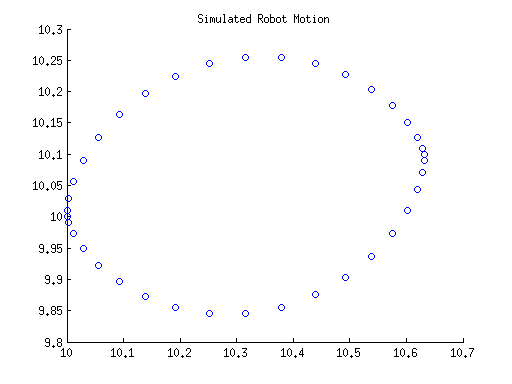
\includegraphics[width=0.75\textwidth]{images/simulatedmotion.png}
\caption{Simulated Motion of Robot}
\end{figure}

\begin{figure}[htp]
\label{fig:simac}
\centering
 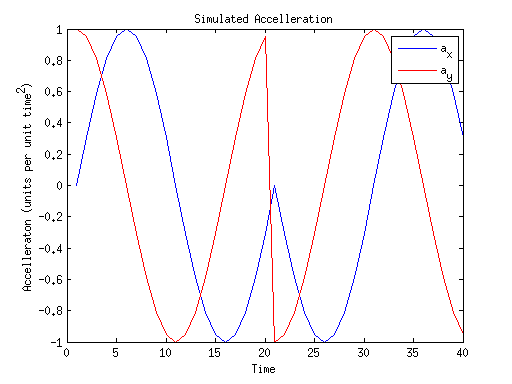
\includegraphics[width=0.75\textwidth]{images/simulatedaccelleration.png}
\caption{Simulated Acceleration of Robot}
\end{figure}

\begin{figure}[htp]
\label{fig:siml}
\centering
 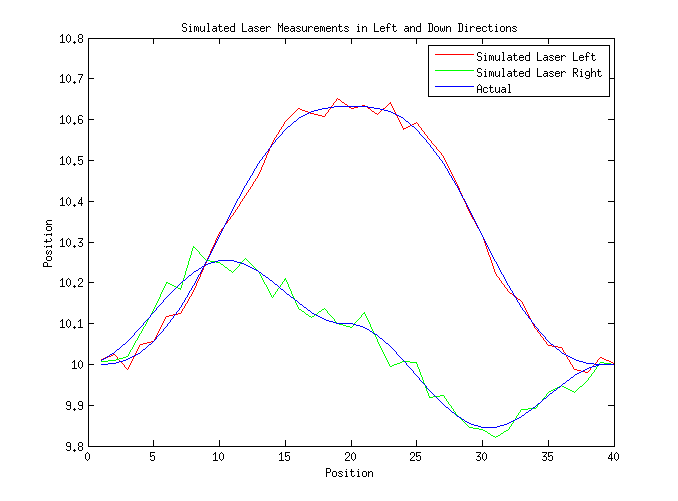
\includegraphics[width=0.75\textwidth]{images/simulatedlaser.png}
\caption{Simulated Noisy Laser Readings}
\end{figure}

Unfortunately, the internal models by which the Kalman Filters and the Particle Filters are constructed precludes a direct comparison of the efficacy of the two algorithms in filtering data, as will be shown below. This means that any further discussion on the merits of one algorithm over the other will be purely based on the authors observations and previous research into the two classes of algorithm.

Each filter was written up in Matlab and processed the same set of data. The ability for the filter to remove the simulated noise was the key metric used in comparing the algorithms.

\subsubsection{The Kalman Filter and Extended Kalman Filter}
As mentioned in section ~\ref{sec:kalfilter}, one of the primary pitfalls of using a simple Kalman Filter in robotics algorithms is the fact that the measurement and movement models are linear functions. This restriction severely limits the type of information which can be incorporated into the filter.

As a result, the Kalman filter implementation focused only on a limited subset of the inputs due to the requirement that the models be linear. Specifically, the implementation focused only on synthesizing the acceleration data ($a_x, a_y$), and two of the range finder measurements($d, l$), those pointing down and to the left. These measurements, you will note, translate directly into the position of the robot, assuming the coordinate system has its origins located at the bottom left of the map. The pose of the robot was represented by position and velocity ($x, y, v_x, v_y$).

The state matrices are therefore given by:
\begin{eqnarray}
A &=& \left[ \begin{array}{cccc}
1 & 0 & \delta t & 0 \\
0 & 1 & 0 & \delta t \\
0 & 0 & 1 & 0 \\
0 & 0 & 0 & 1\end{array} \right] \\
B &=& \left[ \begin{array}{cc}
\frac{\delta t^2}{2} & 0 \\
0 & \frac{\delta t^2}{2} \\
\delta t & 0 \\
0 & \delta t \end{array} \right] \\
C &=& \left[ \begin{array}{cccc}
1 & 0 & 0 & 0 \\
0 & 1 & 0 & 0 \end{array} \right]
\end{eqnarray}

The covariances of the measurements are given to be:
\begin{eqnarray}
R &=& \mathrm{A\_DEV} * \left[ \begin{array}{cccc}
1&0&0&0\\
0&1&0&0\\
0&0&1&0\\
0&0&0&1 \end{array} \right] \\
Q &=& \mathrm{L\_DEV} * \left[ \begin{array}{cc}
1&0\\
0&1 \end{array} \right]
\end{eqnarray}
where A\_DEV and L\_DEV are parameters of the robot that is being investigated. In our case, it is found that the values are given by:
\begin{eqnarray}
\mathrm{L\_DEV} &=& 0.1 \\
\mathrm{A\_DEV} &=& 0.1
\end{eqnarray}

It is assumed that at time $t=0$ the robot is located at the point $(10, 10)$ with zero velocity with complete certainty. We note that this reduces the problem that is being evaluated in this situation to the first class of localization problem, namely that of \emph{Position Tracking}.

By using an Extended Kalman Filter, it is possible to include the parameters that were omitted, as the EFK allows for arbitrary state transition functions $A=g(x), B=h(x)$, which are linearized in the evaluation of the Kalman Filter. By utilizing this form of filter, it is possible to include the missing information, namely the other two range finder's data ($u, r$), pointing in the up and the right direction.

In this case, we consider modifications to two of the main functions. The control(/time) update is performed virtually identically to before, where we calculate $\overline{\mu}_t$ to be linearly dependant on the measured acceleration of the system. However, given the non-linearity present in the measurement step, we must apply the function and linearize to obtain the correct result.

In this case, define:
\begin{equation}
h(x) = \left[ \begin{array}{cccc}l&20-r&d&20-u\end{array}\right]
\end{equation}

The Jacobian of this matrix of the system is then given by:
\begin{equation}
H = \left[ \begin{array}{cc}
1&0\\
-1&0\\
0&1\\
0&-1\\ \end{array} \right]
\end{equation}

Given that the uncertainties are the same as those for the Kalman Filter, we have enough information to apply the Extended Kalman Filter algorithm.

\subsubsection{Particle Filter}
The definition of the particle differs from that of the Kalman filter in a number of key areas. First off, the particle filter aims to solve the Global Localization problem, as opposed to the Tracking problem that the Kalman filter algorithm presented above attempted to solve. As before, the same situations were used, including the same measurement uncertainties, which led to a simple implementation based trivially around the sensor inputs.

The state change probability was sampled around a distribution defined by:
\begin{eqnarray}
V_t &\sim& \mathcal{N}(v_{t-1} + u_{a,t-1}*\delta t, A_DEV) \\
X_t &\sim& \mathcal{N}(x_{t-1} + v_t*\delta t, A_DEV)
\end{eqnarray}

The weighting function then measures the probability given the following distribution:
\begin{eqnarray}
P(\mu_t | z_t) &=& P(\mu_t | u_t, d_t, l_t, r_t) \\
 &=& P(\mu_t | u_t) P(\mu_t | d_t) P(\mu_t | l_t) P(\mu_t | r_t)
\end{eqnarray}

Since we know the laser measurements are distributed normally around (eq. \ref{eq:las} the actual value, it becomes a trivial matter to calculate, given the assumption that $u, d, l, r$ are all independent of each other. Note that in eq. \ref{eq:las}, $x_{t}$ is taken to be the true pose of the robot.

\begin{equation}
\label{eq:las}
p(z_t) \sim \mathcal{N}(x_t, \mathrm{L\_DEV})
\end{equation}

The metric used to determine the accuracy of the obtained results was the RMSE (root mean square error) (eq. ~\ref{eq:rmse}) algorithm, which quantitatively describes the error of each pose estimate, and hence allows comparison of states. In order to counteract the random noise introduced by producing the particle filter representation, the error for each time step was determined as the average RMSE errors over multiple iterations of the algorithm. In our case the values were averaged over 100 iterations of the algorithm.

\begin{equation}
\label{eq:rmse}
\mathrm{RMSE}(x, x_a) = \sqrt{\frac{\sum^n_{i=1} \left(x_i - x_{a,i}\right)^2}{n}}
\end{equation}

% Discuss Kidnapped Robot Problem Implementation.
% Discuss SLAM Implementation

\section{Results}
% Diagram of Kalman, EKF. Diagram RMSE.
% Diagram of Particle Filter. Diagram RMSE.
% Results of Kidnapped Robot.
% Results of FastSLAM

\section{Discussion}

Bayes Filter (Algorithm \ref{alg:bayes}) provides a mathematical algorithm for calculating $bel(x_t)$; however, in general, it is not Turing-computable or is otherwise impractical \cite{probrob}. By assuming $x_t$ may be represented by a Gaussian distribution and that state transitions are linear, the Kalman Filter provides a practical implementation of the Bayes Filter. Furthermore, by representing the belief distribution as a set of state samples which can be individually updated, the Particle Filter provides an alternate practical implementation of Bayes. Both of these algorithms, in general, run in a much shorter amount of time.

In most applications the Kalman Filter is $O(k^{2.4} + n^2)$ where $n$ is the dimension of the state vector and $k$ the dimension of the measurement vector\cite{probrob}. As the filter consists almost entirely of matrix operations, which has been the subject of intense research, it can be implemented using a number of very efficient algorithms for matrix arithmetic. However, the $O(n^2)$ leads to significant scalability issues in high dimensional spaces making performance beyond a few thousand features poor in most modern implementations \cite{Thrun02d}.

The time complexity of certain particle filter implementations can achieve $O(M \log n)$\cite{Thrun02d}. Consequently, particle filters scale far better to high dimensional problems. As the filter only asymptotically produces the correct distribution, too few particles may produce inaccurate or misleading reasults. Nonetheless, as performance is linear in $M$, the algorithm can be efficiently scaled to the desired degree of accuracy.

The assumption by the Kalman Filter that the posterior can be represented by a Gaussian only produces meaningful results for unimodal distributions. However, multi-modal distributions commonly occur in applications such as SLAM as there may exist multiple hypotheses. In these cases, the Kalman filter will produce a belief which is a linear combination of the modes of the distribution. Consequently, a belief may be produced that is impossible or otherwise meaningless within the parameters of the problem. This limits its use in those cases where multiple beliefs are equally likely, or when there is not yet enough information to determine one particular state.

The Particle Filter is equally applicable to multi-modal and unimodal distributions, though a large $M$ may be needed for accurate results if the distribution consists of many alternate hypotheses or the model has a high dimensionality. Consequently, Particle Filters are readily applicable for purposes such as SLAM, as there commonly may exist multiple valid hypotheses before sufficient information has been collected to resolve the correct mode. 

For multi-modal distributions, the Kalman Filter is inapplicable as presented; however it may be adapted to handle multiple hypotheses by representing the posterior as the normalised sum of individual Gaussians in a Multi-Hypothesis Kalman Filter (MHKF)\cite{probrob}.
%Disadvantages of MHKFs?

The Kalman Filter also cannot incorporate negative information (i.e. the lack of an expected observation) as this can neither be represented by a gaussian nor a linear combination of gaussians \cite{Thrun02d}. As Particle Filters can asymptotically represent an arbitrary distribution, they do not suffer from this drawback.

The Kalman Filter is dependent on the linearity of the measurement and movement models; in few practical applications does this assumption hold. Consequently, the basic Kalman Filter is of limited practical utility. This may be overcome by  modifying the algorithm to conditionally apply a different model based on the prior probability distribution (i.e. treat the models as piecewise-linear functions). Alternatively, the Extended Kalman Filter (EKF) allows the models to be arbitrary smooth functions and uses the first-order Taylor expansion to linearize the function for the state update. The EKF can be considered a generalisation of the first solution. Due to the linearisation of the functions, the EKF is highly sensitive to nonlinearities (i.e significant higher order terms). This degree of sensitivity is highly dependent on the uncertainty of the prior\cite{probrob}. Consequently, though the EKF is widely used in practice\cite{probrob}, it is ill-suited to applications with significant non-linearities in the measurement and movement models and large uncertainties.

% Discuss accuracy results for actual measurements.

% Discuss results of Kidnapped Robot Problem

% Discuss results of FastSLAM

\section{Conclusion}

\bibliographystyle{plain}
\bibliography{references}

\end{document}
